\section{Custom Hardware}

\textbf{Instruction power efficiency}
Many instructions have a large overhead, the an entire instruction can take up to
70pJ, but the operation might take ~0.5pJ, meaning that the overhead is 99\%. To
solve this we can amortize instructions by performing a large number of operations
per instruction, and for each data cache access

\textbf{Data-Level Parallelism} We can use \textbf{vector} instructions to do a
single operation on many values. To do this we need to add vector registers, as
set a small values.
\begin{verbatim}
    vadd.vv v3, v1, v2
\end{verbatim}

\textbf{SIMD} single instruction muliple data instructions.

\textbf{FPGA's} are Field-programmable Gate Arrays, they are 2-D arrays of reconfigurable
logic elements. They are used for digital circuit emulation and as custom hardware
accelerators

\textbf{Multicore} In a multicore system we encounter the problem of synchronizing
data, to fix this we can lock parts of memory when we are modifying it, and then
unlock it when we are done.

\textbf{Multithreading} When we are multithreading we execute multiple threads
on a single core, threads within a process will have separate PC and registers,
but will share the same virtual memory space. When 1 thread stalls, switch to
another thread.

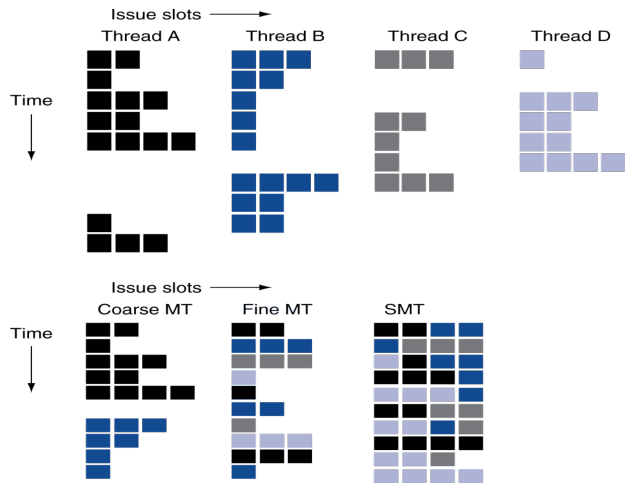
\includegraphics[width=\linewidth]{png/multithread.png}
